\documentclass{beamer}
\usepackage[utf8]{inputenc}
\usepackage{amsfonts}
\usepackage{amssymb}
\usepackage{amsthm}
\usepackage{amsmath}
\usepackage{amsopn} 
\usepackage{sansmathaccent}
\usepackage{bookmark}
\usepackage{mathtools}
\usepackage{tikz}

\usebackgroundtemplate{
\tikz\node[opacity=0.3]{
\includegraphics[width=\paperwidth,height=\paperheight]{1a9c7eb96139cf036f1991bd5f207a69}};}
\usetheme{Antibes}
\usecolortheme{seahorse}
\title{Kratka predstavitev}
\subtitle{\textbf{DOMEL HOLDING D.D. - Posebnosti pri vrednotenju podjetja z internim trgom delnic}}
\author{\textbf{avtorica: Neža Habjan\\
mentor: doc. dr. Matjaž Črnigoj}}

\institute{\textbf{Fakulteta za matematiko in fiziko}}
\date{\textbf{\today}}
\begin{document}
\begin{frame}
\titlepage
\tableofcontents
\end{frame}

%\usebackgroundtemplate{}
\begin{frame}
\frametitle{DOMEL - PREDSTAVITEV PODJETJA}
\begin{itemize}
\item Večje slovensko industrijsko podjetje - 1946, sedež v Železnikih, 1237 zaposlenih (2017)
\item Proizvodnja el. motorjev in komponent iz laminatov, aluminija, termo plastike in BMC duroplasta
\item Področje vakuumskih enot, bele tehnike, prezračevanja, medicine, avtomobilske proizvodnje,...  % el. motorji za suho in mokro sesanje
\item Tuj trg: \textbf{\textcolor{red}{Nemčija}}, Madžarska, Švedska, Poljska, Italija, Avstrija, Romunija %podružnici - Kitajska, ZDA
\item V Evropi \textbf{60$\%$ tržni delež} na področju sesalnih enot (Elektrolux, Philips, Rowenta, Stihl, Husqvarna, Samsung...) %V 6 od 10 v Evropi prodanih sesalnikov je vgrajen motor izdelan v podjetju Domel
\end{itemize}
\end{frame}


\begin{frame}
\begin{center}
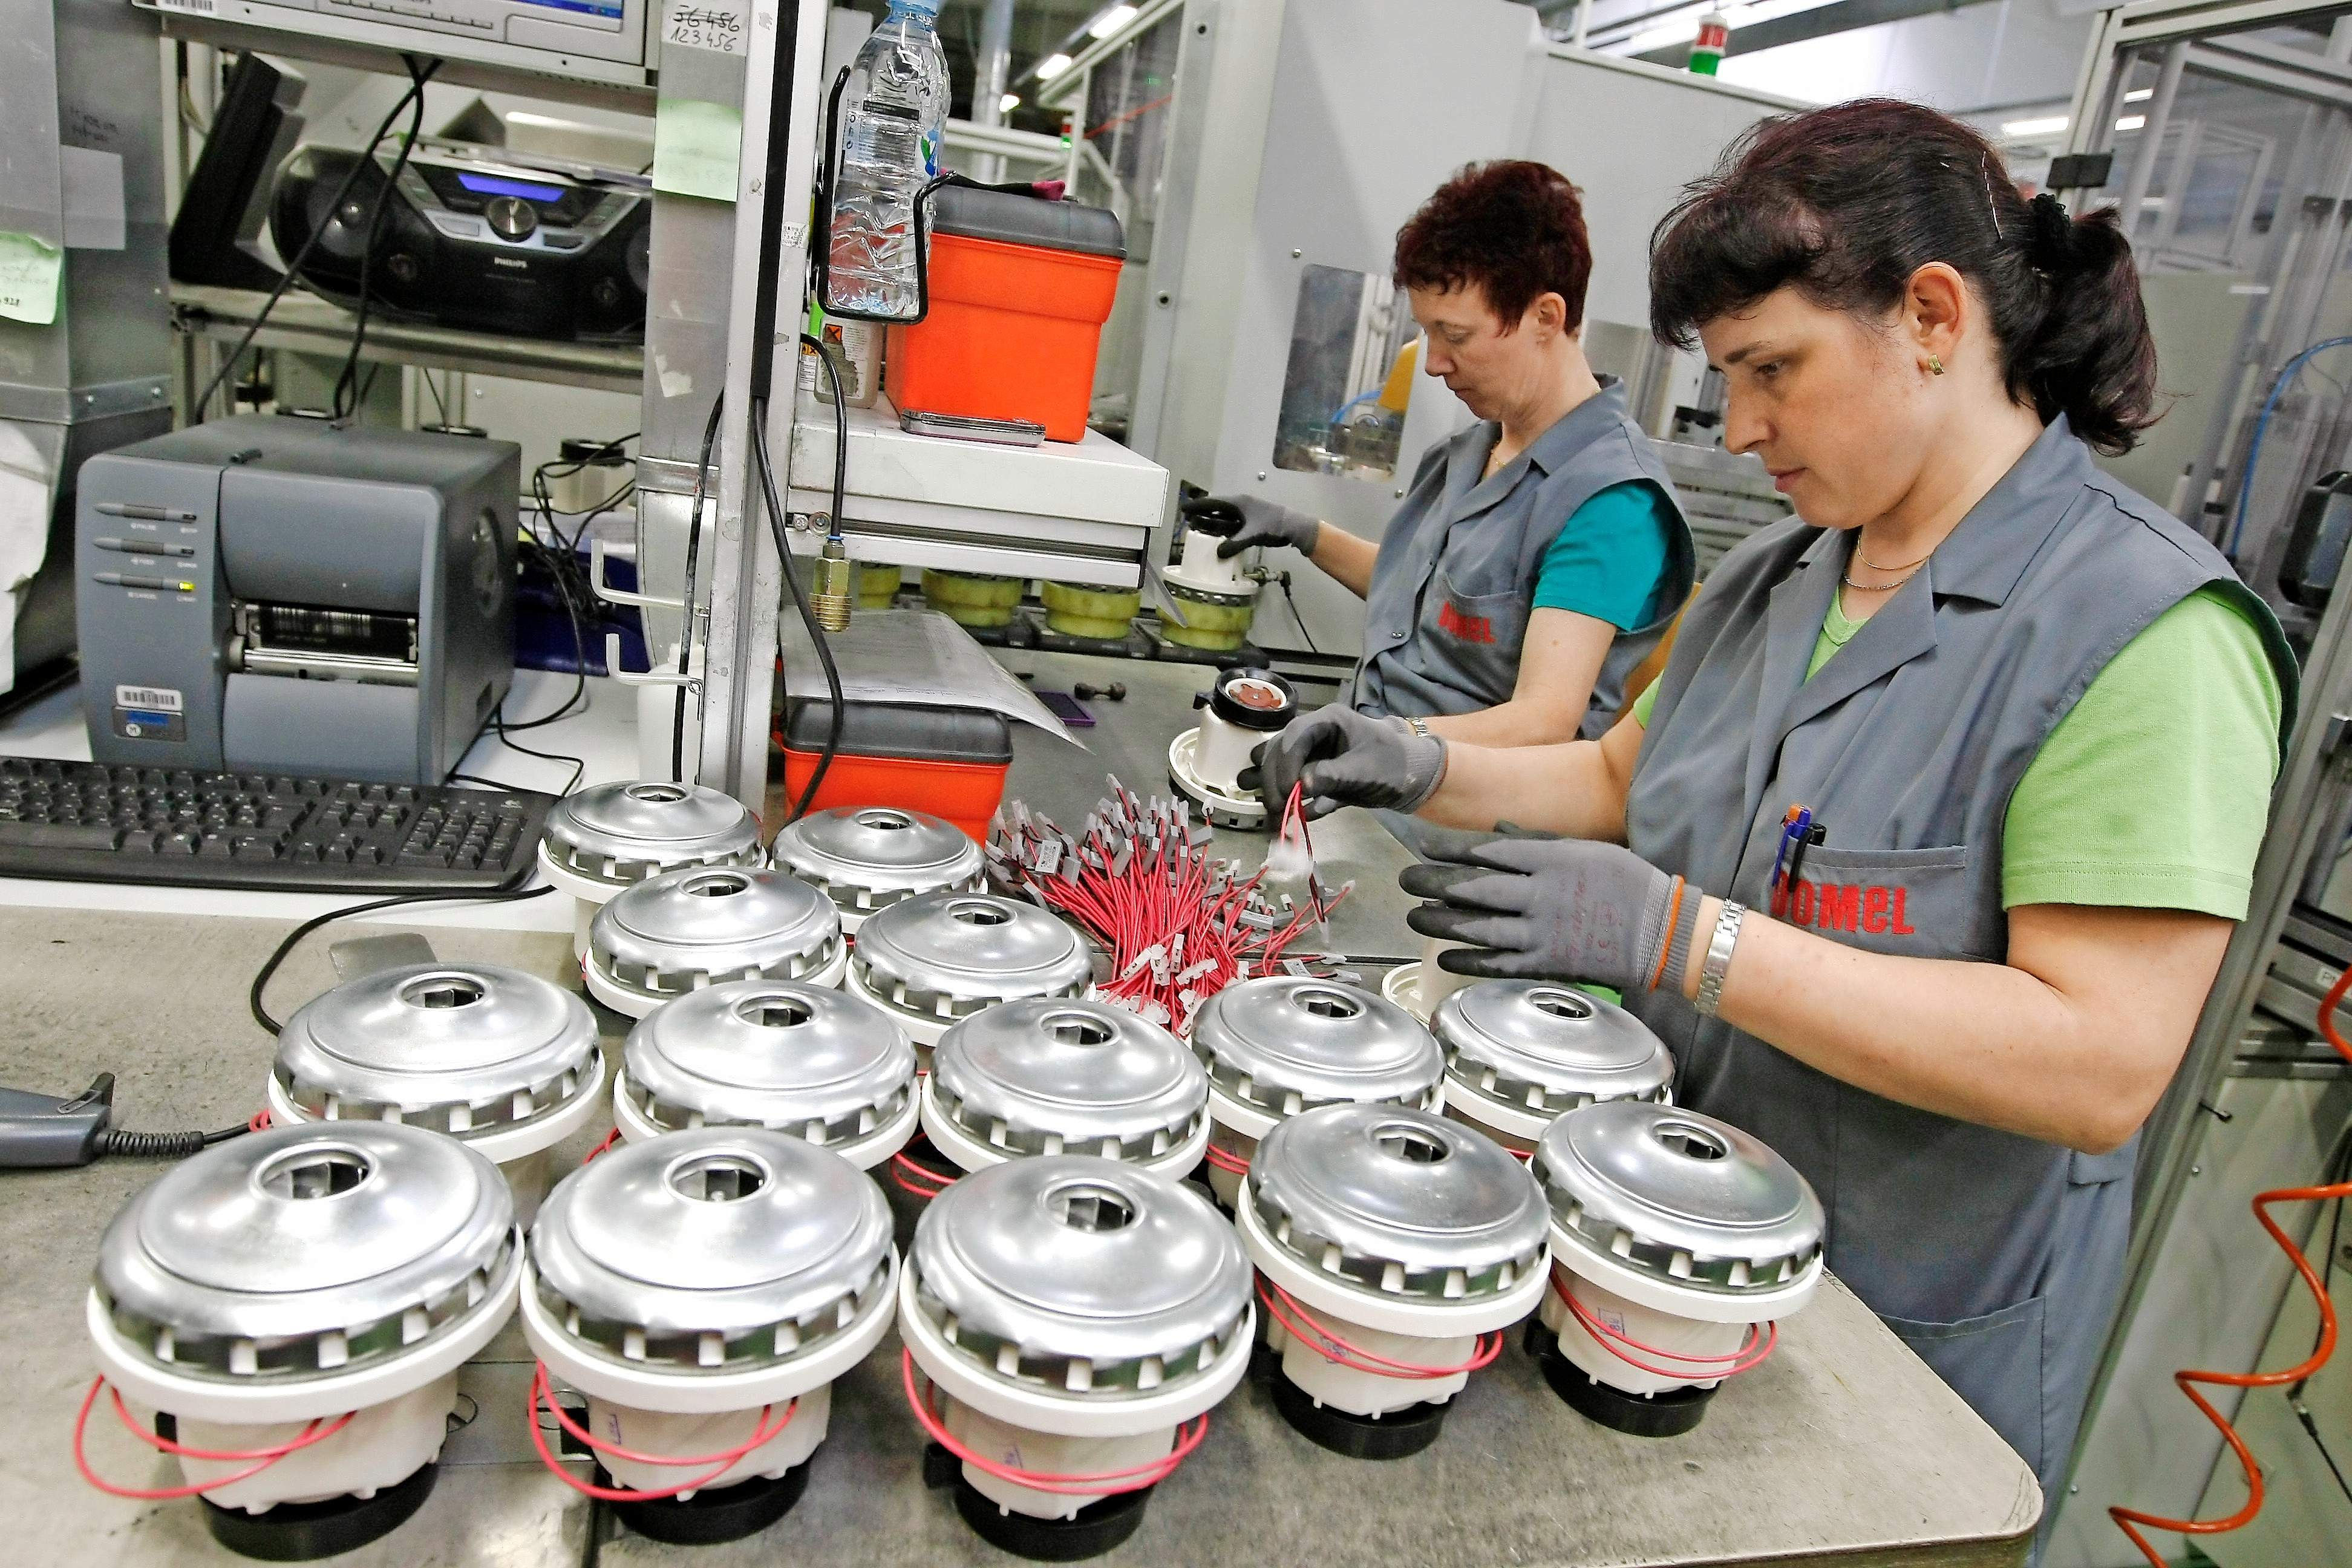
\includegraphics[scale=0.22]{_home_datadisk_arhiv_assets_transfer_images_web_201407_18_140719835-AR_1}
\end{center}
\end{frame}


%\begin{frame}
%\frametitle{KRATKA ZGODOVINA IN ZASNOVA PODJETJA}
%\begin{itemize}
%\item 1946 - 1962 : NIKO - kovinski in elektromehanski izdelki
%\item 1962 - 1991 : del podjetja ISKRA
%\item 1991 - Elektromotorji d.o.o. $->$ 1994 - Domel d.d.
%\item 1998 - Ustanovitev Družbe pooblaščenke Domel Holding d.d. (upor zaposlenih proti sovražnemu prevzemu) %uprava želela prodati američanom, nato američani kupili Italijansko podjetje, ki so ga po parih letih zaprli - želeli le povečati svoj tržni delež, na račun Domela
%\item 2010 - Domel d.o.o., danes v 100 $\%$ lasti Domel Holding d.d.
%\item delniška družba z \textbf{internim trgom delnic}
%\end{itemize}
%\end{frame}


\begin{frame}
\frametitle{STRUKTURA DRUŽBE}
\begin{figure}
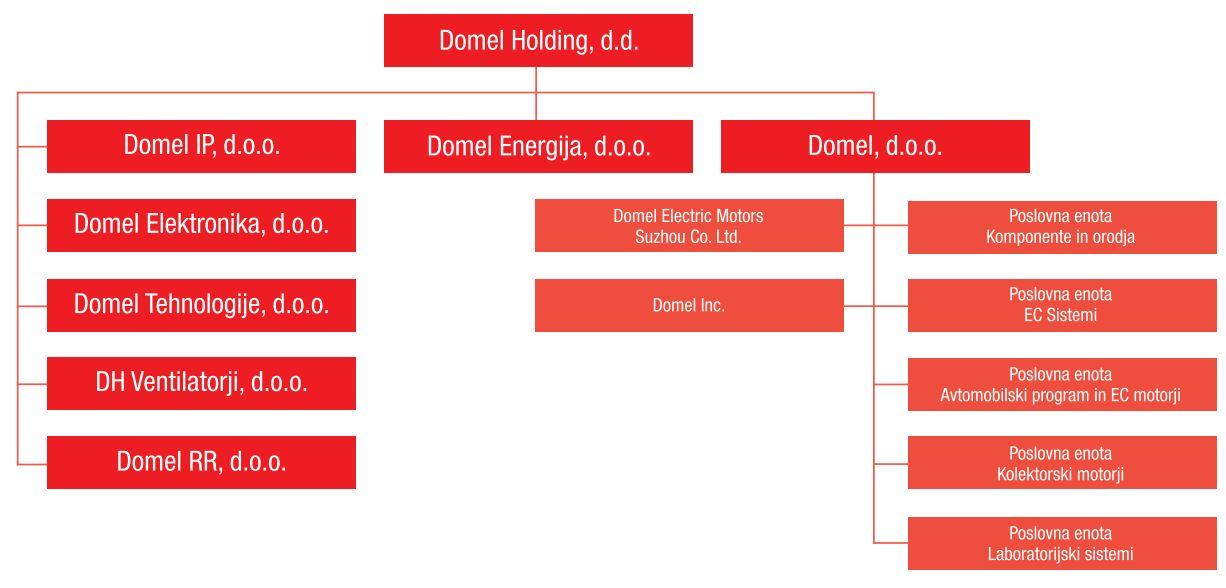
\includegraphics[scale=0.33]{Organigram_Domel_skupina_2018}
\end{figure}
\end{frame}


\begin{frame}
\frametitle{DOMEL - DELNIŠKA DRUŽBA}
\begin{itemize}
\item osnovni kapital je razdeljen na \textbf{delnice} - delničarji sprejmejo statut
\item dvotirni sistem upravljanja - uprava in nadzorni svet
\item lastniki delnic: pravica do izplačila dividend + do soupravljanja družbe (1 delnica - 1 glas)
\end{itemize}
\end{frame}


%\begin{frame}
%\frametitle{PREDNOSTI IN SLABOSTI}
%\begin{itemize}
%\item \textbf{prednosti:}
%\begin{itemize}
%\item družbenik za obveznosti \textbf{\textcolor{red}{ne odgovarja osebno}}, pač pa družba do višine lastnega premoženja
%\item možnost delovanja \textbf{\textcolor{red}{na borzi}}
%\item sklepanje pravnih poslov med družbo in njenimi družbeniki
%\end{itemize}
%\item \textbf{slabosti:}
%\begin{itemize}
%\item dolžnost vplačila osnovnega kapitala (25.000 EUR) - za zagon podjetja, jamstvo upnikom, osnova za izračun korporacijskega deleža delničarja
%\item izplačevanje dividend davčno obremenjeno
%\item zahtevnejši postopek ustanovitve
%\end{itemize}
%\end{itemize}
%\end{frame}


\begin{frame}
\frametitle{DRUŽBA POOBLAŠČENKA DOMEL}
\begin{itemize}
\item ustanovljena zaradi strahu pred domnevnim sovražnim prevzemom
\item delavci, člani pooblaščenke, odkupujejo delnice - danes skupaj večinski lastniki podjetja
\item  \textbf{nizke cene delnic} (neizpostavljene trgu) - zato za kompenzacijo visoke dividende  
\end{itemize}
\end{frame}


\begin{frame}
\frametitle{LASTNIŠTVO V DOMELU (31.12.2017)}
\textbf{INTERNI TRG DELNIC:}
\begin{itemize}
\item zaposleni (52,66$\%$)
\item bivši zaposleni (9,06$\%$)
\item upokojenci (30,51$\%$)
\item ostali (7,04$\%$) - delnice vplačane z denarjem, ki niso nujno del pooblaščenke
\end{itemize}
Osnovni kapital: 2.145.781 EUR, sestavljen iz \textbf{514.215} delnic z nominalno vrednostjo 4,1729 EUR. 
Lastnih delnic 0,13\% osnovnega kapitala (maksimum je 10 \%)
(Lastne delnice - kupljene delnice obvladujoče družbe Domel Holding, d.d.)
\end{frame}


\begin{frame}
\frametitle{DELNICE DRUŽBE POOBLAŠČENKE DOMEL}
\begin{itemize}
\item \textbf{navadne delnice (A):}
\begin{itemize}
\item v 30 dneh prodaje delnice Družba pooblaščenka dobi predkupno pravico
\item za prodajo tretji osebi potrebno soglasje nadzornega sveta
\end{itemize}
\item \textbf{denarno vplačane delnice (B):}
\begin{itemize}
\item prvo pravico nakupa ima Družba pooblaščenka (30 dni)
\item sicer za prodajo tretji osebi soglasje nadzornega sveta ni potrebno
\end{itemize}
\end{itemize}
\end{frame}


\begin{frame}
\begin{center}
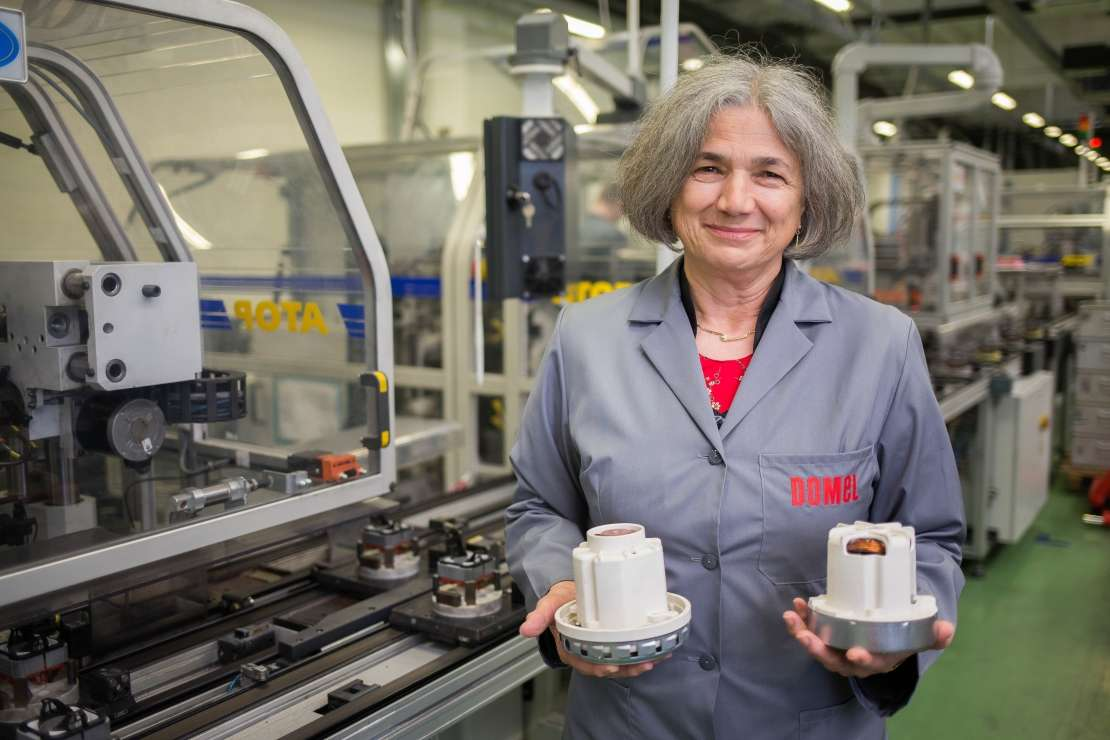
\includegraphics[scale=0.27]{0e42aea7180eca92ec1ca673c0788f78}
\end{center}
\end{frame}


\begin{frame}
\frametitle{OCENA VREDNOSTI PODJETJA}
\begin{enumerate}
\item \textbf{Vrednotenje na podlagi tržne primerjave} $->$ primerljiva so podjetja, ki nastopajo na relevantnih trgih s podobnimi značilnostmi glede stopnje tveganja, s podobnim blagom oziroma storitvami in primerljivo velika, s podobnim poslovanjem v preteklosti in podobnim trgom. %primerljivo podjetje bi težko našla, zaradi specifike lastništva Domela
\end{enumerate}
\end{frame}


\begin{frame}
\frametitle{OCENA VREDNOSTI PODJETJA}
\begin{enumerate}[2]
\item \textbf{Metoda čiste vrednosti sredstev:}
\begin{block}{Izračun:}
vrednost dolgoročnih in kratkoročnih sredstev - vrednost dolgoročnih in kratkoročnih obveznosti
\end{block}
\begin{itemize}
\item za podjetja z veliko knjigovodsko zabeleženih sredstev (ne znanstveniki - inteligenca...)
\item upoštevamo tržne vrednosti sredstev - nadomestitveno vrednost naložbe za kupca
\end{itemize}
\end{enumerate}
\end{frame}


\begin{frame}
\frametitle{OCENA VREDNOSTI PODJETJA}
\begin{enumerate}[3]
\item \textbf{Diskontiranje prihodnjih denarnih tokov} (predpostavka poslovanja v neskončost)
\begin{block}{Formula:}
      $$PV=\frac{CF1}{1+r}+\frac{CF2}{(1+r)^2}+\frac{CF3}{(1+r)^3}+\ldots+\frac{CFn}{(1+r)^n}+\frac{\frac{CFn*(1+g)}{r-g}}{(1+r)^n}$$
\end{block}
\begin{itemize}
\item r: disk. faktor - tveganje in časovna vrednost denarja
\item g: stopnja rasti podjetja
\item najbolj korektna in natančna
\item zahteva napoved poslovanja in \textbf{diskontne stopnje}
\end{itemize}
\end{enumerate}
\end{frame}


\begin{frame}
\frametitle{OCENA VREDNOSTI PODJETJA}
\underline{Določanje diskontnega faktorja:}\\
\begin{itemize}
\item \textbf{CAPM model: $$R=Rn+\beta*Rt+Rm+Rd+Rp$$}
 Rn - mera donosa netveganega vrednostnega papirja na dan vrednotenja\\
 Rt - pribitek za kapitalsko tveganje
 beta - tveganost podjetja v primerjavi z drugimi iz iste panoge\\
 Rm -  pribitek za majhnost\\
 Rd - pribitek za deželno tveganje (če delnica ni iz slovenskega podjetja)\\
\end{itemize}
\end{frame}


\begin{frame}
\frametitle{OCENA VREDNOSTI PODJETJA}
\begin{itemize}
\item \textbf{WACC tehtani povprečni stroški kapitala: $$WACC=(Ke*We)+(Kp*Wp)+(Kdp*(1-t)*Wd)$$}
 Ke - strošek kapitala pri navadnih delnicah\\
 We - odstotek kapitala v navadnih delnicah\\
 Kp - strošek kapitala pri prednostnih delnicah\\
 Wp - odstotek kapitala v prednostnih delnicah\\
Kdp - strošek dolga pred obdavčitvijo\\
 t - davek\\
 Wd - delež kapitala financiranega z dolgom\\
\end{itemize}
\end{frame}


\begin{frame}
\frametitle{PROBLEM NALOGE}
\begin{itemize}
\item poračunana vrednost po metodi diskontiranja NI realna - \textbf{vpliv zaprtega trga delnic}
\item upoštevati bo potrebno odbitke in pribitke: %zelo velik vpliv na končno vrednost
\begin{itemize}
\item odbitek zaradi \textbf{neobvladovanja podjetja} - preučujem vrednost za manjšinskega lastnika
\item odbitka zaradi \textbf{pomanjkanja tržljivosti} in zaradi \textbf{nelikvidnosti}
\end{itemize}
\item odbitek izrazimo kot dodane procentne točke diskontnemu faktorju $->$ nižja sedanja vrednost investicije
\end{itemize}
\end{frame}


\begin{frame}
\frametitle{GLAVNA KONCEPTA ZA UGOTAVLJANJE ODBITKA}
\begin{itemize}
\item \textbf{TRŽLJIVOST}: izraža delovanje trga, kako hitro lahko prodamo lastniški delež in prejmemo denar
\begin{itemize}
\item delujoč in aktiven trg
\item preko empiričnih študij
\item analize dejavnikov, ki vplivajo na stopnjo tržljivosti (pravica prodaje, potencialni kupci, dividendni donos, pričakovanost kotacije na borzi,...)
\end{itemize}
\end{itemize}
\end{frame}


\begin{frame}
\frametitle{GLAVNA KONCEPTA ZA UGOTAVLJANJE ODBITKA}
\begin{itemize}
\item \textbf{LIKVIDNOST}: zmožnost lastnika, da obrne sredstva ali vrednostne papirje v denar, brez večjih transakcijskih stroškov
\begin{itemize}
\item v primeru poplačila dolga
\item preko kazalcev likvidnosti (kratkoročna sredstva/kratkoročne obveznosti)
\item višja likvidnost zmanjša tveganost naložbe
\end{itemize}
\end{itemize}
\end{frame}


%\begin{frame}
%\frametitle{VREDNOST DELNICE}
%\begin{itemize}
%\item \underline{knjigovodska vrednost}: vrednost kapitala/število delnic %običajno večja od nominalne, tudi različna od tržne (ta vključuje še pričakovanja vlagateljev v prihodnosti
%\item \underline{nominalna vrednost}: vrednost osnovnega kapitala/število delnic %v sloveniji minimalno 1 euro
%\item \underline{notranja vrednost}: izračun preko vrednotenja podjetja - nanjo vplivajo:
%\begin{itemize}
%\item uspešnost poslovanja in pričakovana rast v prihodnosti
%\item raven obrestnih mer v gospodarstvu (stroški financiranja)
%\item tveganost - zahtevana donosnost delnice
%\item delež dobička, ki je izplačan v dividendah
%\end{itemize}
%\item \underline{tržna vrednost}: koliko so vlagatelji za delnico pripravljeni plačati
%\end{itemize}
%\end{frame}


\begin{frame}
\frametitle{CILJ IN NAMEN NALOGE}
\begin{itemize}
\item \textbf{določiti ustrezen diskontni faktor za vrednotenje podjetja preko prihodnjih denarnih tokov}
\item določiti vrednost delnice podjetja Domel, z upoštevanjem odbitkov
\item preučiti vpliv tržljivosti in likvidnosti v podjetju Domel na prodajo delnic med delničarji
\item ovreči oziroma potrditi postavljene hipoteze
\end{itemize}
\end{frame}


\begin{frame}
\frametitle{HIPOTEZE IN NAČIN DELA}
\begin{enumerate}
\item \textbf{Podjetje Domel pri vrednotenju delnice izgubi za 40\% vrednosti zaradi odbitkov upoštevanih pri diskontnem faktorju.}
\begin{itemize}
\item Po ugotovljeni vrednosti delnice podjetja, bom z upoštevanjem diskontnega faktorja (prilagojenega za vse odbitke/pribitke), poračunala dejansko vrednost delnice, ki ne kotira na borzi in je izpostavljena le majhnemu internemu trgu.
\end{itemize}
\end{enumerate}
\end{frame}


\begin{frame}
\frametitle{HIPOTEZE IN NAČIN DELA}
\begin{enumerate}[2]
\item \textbf{Težnja po prodaji delnic med delničarji se ob povečevanju čistega dobička podjetja niža.}
\begin{itemize}
\item Z izdelavo ankete med zaposlenimi bi ugotovila kateri so njihovi glavni razlogi za prodajo oziroma odkup delnic, s tem pa bi lažje ocenila kakšna je dejanska tržljivost delnice, torej kako hitro jo delničar lahko proda, brez večjih stroškov. Tržljivost bi upoštevala pri odbitku vrednosti delnice.
\end{itemize}
\end{enumerate}
\end{frame}

%\usebackgroundtemplate{
%\tikz\node[opacity=0.3] {\includegraphics[width=\paperwidth,height=\paperheight]{domeldooelektromotorjiingospodinjskiaparati1-1485874913}};}
\begin{frame}
\begin{center}
\textbf{HVALA ZA VAŠO POZORNOST!}
\end{center}
\end{frame}

\end{document}